\section{Discussion}
\label{sec:flakycat-discussion}



% To further understand these results, we inspect a test that was misclassified by FlakyCat.
% The test is presented in the listing~\ref{fig:test_example}\footnote{https://github.com/apache/hbase/commit/e89712d29dd91be4}.
% Based on the dataset of Luo~\etal~\cite{Luo2014}, the original flakiness label of this test is \textit{Network}, because the test fails intermittently due to a lack of online dependency.
% However, FlakyCat assigns it first to the category \textit{Concurrency}, then the second label is \textit{Async waits}, and the third one is \textit{Network}. Analyzing the whole test, we can notice that it uses multiple threads, unordered collections, and asynchronous wait for a fixed time, so the test may be flaky for other reasons.
% Hence, statically multiple categories of flakiness can be assigned to it. In this case, the model can't make much of a distinction, because it works with similarities, and the test is similar to more than one category. 
% ~~\\


% \begin{figure}[htbp]
% \centerline{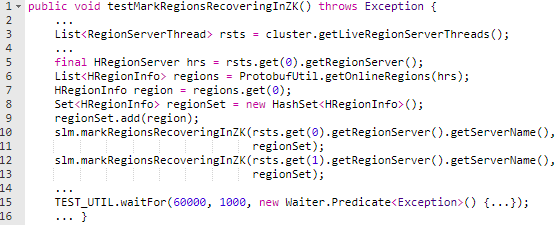
\includegraphics[scale=0.62]{figures/test_example.PNG}}
% \caption{A flaky test from the Category \textit{Network} taken from the project HBase.}
% \label{fig:test_example}
% \end{figure}

\subsection{Reasoning about the statements influencing FlakyCat and the usage of flakiness categories}
\label{sec:discussion:reasoning}

Listing~\ref{lst:flaky-example} gives an example of a flaky test taken from the Neo4J project\footnote{https://github.com/neo4j/neo4j/commit/c77e579b40b02087} found during the data collection part.
As explained in the commit message, the flakiness was caused by a race condition and thus, we affected it to the Concurrency category. FlakyCat classified this test as Async wait. The interpretability technique that we introduced in Section~\ref{sec:flakycat-interpretability} reveals that the statement on line 6 is the most influential for the model's decision. It contains the \texttt{await()} function, and this is likely the reason why the flaky test was categorized as Async wait. Furthermore, similarity score for the Concurrency category is high, and it comes as FlakyCat's second guess. 

When looking at the test, we understand that an asynchronous wait was performed to wait for a thread. We also found similar examples concerning other categories, such as waits relying on network resources. First, we argue that our interpretability technique can help to understand the cause of flakiness, even when FlakyCat apparently mislabelled the test. Secondly, we advance that flakiness categories as commonly defined in research studies~\cite{Luo2014, Eck2019} can overlap, \ie a flaky test can belong to several categories. The application of machine learning to determine the causes of flakiness is promising and should receive attention. It would also benefit from a more precise, orthogonal classification of flakiness categories. \\


\begin{lstlisting}[caption={A flaky test belonging to two categories
},label={lst:flaky-example},language=Java]
@Test
public void shouldPickANewServer[...]() throws Throwable {
[...]
    Thread thread = new Thread( () -> {
    try {
    startTheLeaderSwitching.await();
    CoreClusterMember theLeader = cluster.
        awaitLeader();
    switchLeader( theLeader );
    } catch ( TimeoutException | InterruptedException e ) {
        // ignore
    }});
[...]
}
\end{lstlisting}

% \begin{table*}[htbp]
% \caption{Prevalence of different types of statements in each flakiness category for false positive predictions }
% \begin{center}
% \resizebox{\textwidth}{!}{
% \begin{tabular}{|c|c|c|c|c|c|c|c|c|c|c|}
% \hline
%  & \#Statements &	Control flow &	Constants &	Asserts &	Threads	& Waits &	Network & Global variables &	Usage of Date/time	 & I/O \\
% \hline 

% Async Waits &  22 &	9,09\% &	36,36\%  &	22,73\% &	13,64\%  &	13,64\%  &	27,27\%  &	9,09\% &	9,09\% &	27,27\% \\

% \hline 
% Concurrency & 20 &	25\% &	40\% &	10\% &	30\% &	15\% &	15\% &	5\% &	5\% &	30\%  \\
% \hline 

% test order dependency & 3 &	0\% &	100\%	 & 66,67\% &	0\% &	0\% &	0\% &	0\% &	0\% &	0\% \\

% \hline 

% Time &  4 &	0\% &	50\% &	25\% &	0\% &	25\% &	0\% &	25\% &	25\% &	25\%\\
% \hline 

% Unordered collections & 1 &	0\% &	100\% &	0\% &	0\% &	0\% &	0\% &	0\% &	0\% & 	0\% \\

% \hline
% \end{tabular}
% }
% \end{center}
% \label{TabStatmentsFP}
% \end{table*}
% \vspace{-4mm}

\subsection{The effect of considering an additional category}
Our results showed that flakiness categories can be classified automatically. We carried out our main experiments with five categories of flakiness for which we had a reasonable number of tests. Still, we believe that one interesting aspect of our study is to understand the impact of adding other categories to FlakyCat. 
For this, we investigate the performance of FlakyCat for each category (similarly to RQ2), but we add to our set the \textit{Network} category,
which is the next category with the most samples in our dataset (25 tests). F1 scores and the accuracy obtained for each category are presented in Figure \ref{fig:fsl_add_class}. 

Compared to the results previously reported in Table~\ref{scores}, we observe that the performances of each category are slightly impacted.
The \textit{Async waits} category is the most impacted one. 
Indeed, after adding the \textit{Network} category, we get an overall F1 score of 0.68. The added category gets the worst results. 
This performance drop can be explained by multiple factors.
First, having more categories to differentiate makes it more challenging for FlakyCat to distinguish between them.
% Indeed, the top five categories become more difficult to distinguish, which means that the added category have common characteristics with them. 
Secondly, the overall F1 score is strongly affected by the poor performance observed in the new category.
The performance for the Network category can be a result of the too low number of examples in this category (25). Despite using FSL, the model still requires enough data points in each category. While collecting data, we noticed that flaky tests caused by Network were not common. These findings align with the ones about the prevalence of the different categories reported in previous empirical studies~\cite{Luo2014,Eck2019}. In addition, flaky tests related to \textit{Network} issues could also be considered as Asynchronous waits in many cases, as previously explained. 


\begin{figure}[htbp]
\centering
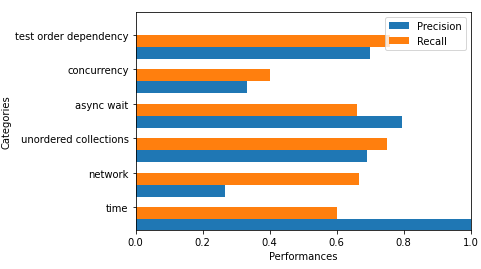
\includegraphics[scale=0.8]{figures/flakycat/add_network.PNG}
\caption{Precision and Recall per flakiness category when adding the category "Network" }
\label{fig:fsl_add_class}
\end{figure}
\vspace{-2mm}

% The results of RQ3 highlight the type of code statements on which our model relies to make predictions. Looking at these results, we can notice that, according to the model, \textit{Async waits} and \textit{Concurrency} categories have similar types of statements behind them.
% These statements are related to the use of threads, wait statements with fixed time values, constants and external calls. This means that the two categories have common characteristics. Moreover, external calls, including network calls which constitute a separate flakiness category, are also frequent in the \textit{Async waits} and \textit{Concurrency} categories. In addition, time-related statements, which are mainly present in the \textit{Time} flakiness category, occur also in the \textit{Async waits} and \textit{Concurrency} categories. This implies that several defined flakiness categories can intersect (or be included in one another). The results may also draw our attention to the fact that even some elements of the code that may seem important when debugging flakiness problems may be part of the problem. As table~\ref{TabStatments} shows, constants and asserts are among the important elements for the classification of the categories \textit{Time} and \textit{Unordered collection}. This is because flaky tests that are caused by unordered collection try to assert that elements of an unordered collection are exactly equal to constant values with a fixed order.
% The same issue occurs in the \textit{Time} category as tests compare time values with different precision.
% This means that developers and tools should be careful with exact equality assertions to avoid these categories of flakiness.
 





% \paragraph{Limits}
% Another threat happens when we ask our model to classify a test from an unsupported category. In this case, the model can only give one of the category it was trained on. Still, we believe flakiness categories are not orthogonal and that it is possible for a flaky test to belong to several categories. For example, a flaky test relying on network or I/O can flake because of an asynchronous wait. Thus, we consider that the prediction of our model can still provide value to understand the root cause in those cases. 
% One limit of our approach is derived from the use of CodeBERT. To get its CodeBERT representation, the number of tokens in a test can't exceed 512. When collecting our data, tests were discarded when they were too long. We can't guarantee that our approach would generalize to longer and higher level tests. The same applies for other languages.